%!TEX root = ../thesis.tex

\section{実験の概要}
開発した経路追従ソフトウェアを実環境で検証する.
AI-Formulaの会場となっているAIモビリティパーク紫峰で実験を行う.
Fig.6.1にAIモビリティパーク紫峰を示す.
検証をするにあたって, いくつかの評価項目を設ける. 
評価項目をTable.6.1に示す.
追従誤差は目標経路の全ての経路点とGNSSから得たモビリティの座標データの距離から最小の値を取り出すことで求める.
求めた追従誤差を積分することで, 積分絶対値誤差を求める.

\begin{table}[H]
  \centering
  \caption{Evaluation item}
  \begin{tabular}{cclll}
  \cline{1-1}
  評価項目                    &  &  &  &  \\
  \cline{1-2}
  目標速度(並進速度) {[}m/s{]}    &  &  &  &  \\
  ゴールするまでの時間 {[}s{]}            &  &  &  &  \\
  積分絶対値誤差 {[}m·s{]} &  &  &  &  \\
  追従誤差の最大値 {[}m{]}  &  &  &  &  \\
  \multicolumn{1}{l}{}    &  &  &  &  \\
  \multicolumn{1}{l}{}    &  &  &  & 
  \end{tabular}
\end{table}

% \section{実験環境}
% 本実験では茨城県常総市にあるAIモビリティパーク紫峰にて行う.
% AIモビリティパーク紫峰は平坦な地形であり, アスファルト舗装された路面や車線などの路面情報が整備されているコースである.

\begin{figure}[H]
  \centering
 \includegraphics[keepaspectratio, scale=0.1]
      {images/AerialViewAndMobilitysPerspetiveOfTheCourse.png}
 \caption{Aerial view and mobility perspective of the course}
 \label{fig:course}
\end{figure}

\section{実験装置}
実験装置をFig6.2に示す.
センサ類はGNSS+IMUセンサ(VectorNav VN-200)を使用する.
また, 実験の様子を空撮するためにドローン(DJI Air3)を使用した.

\begin{figure}[H]
  \centering
 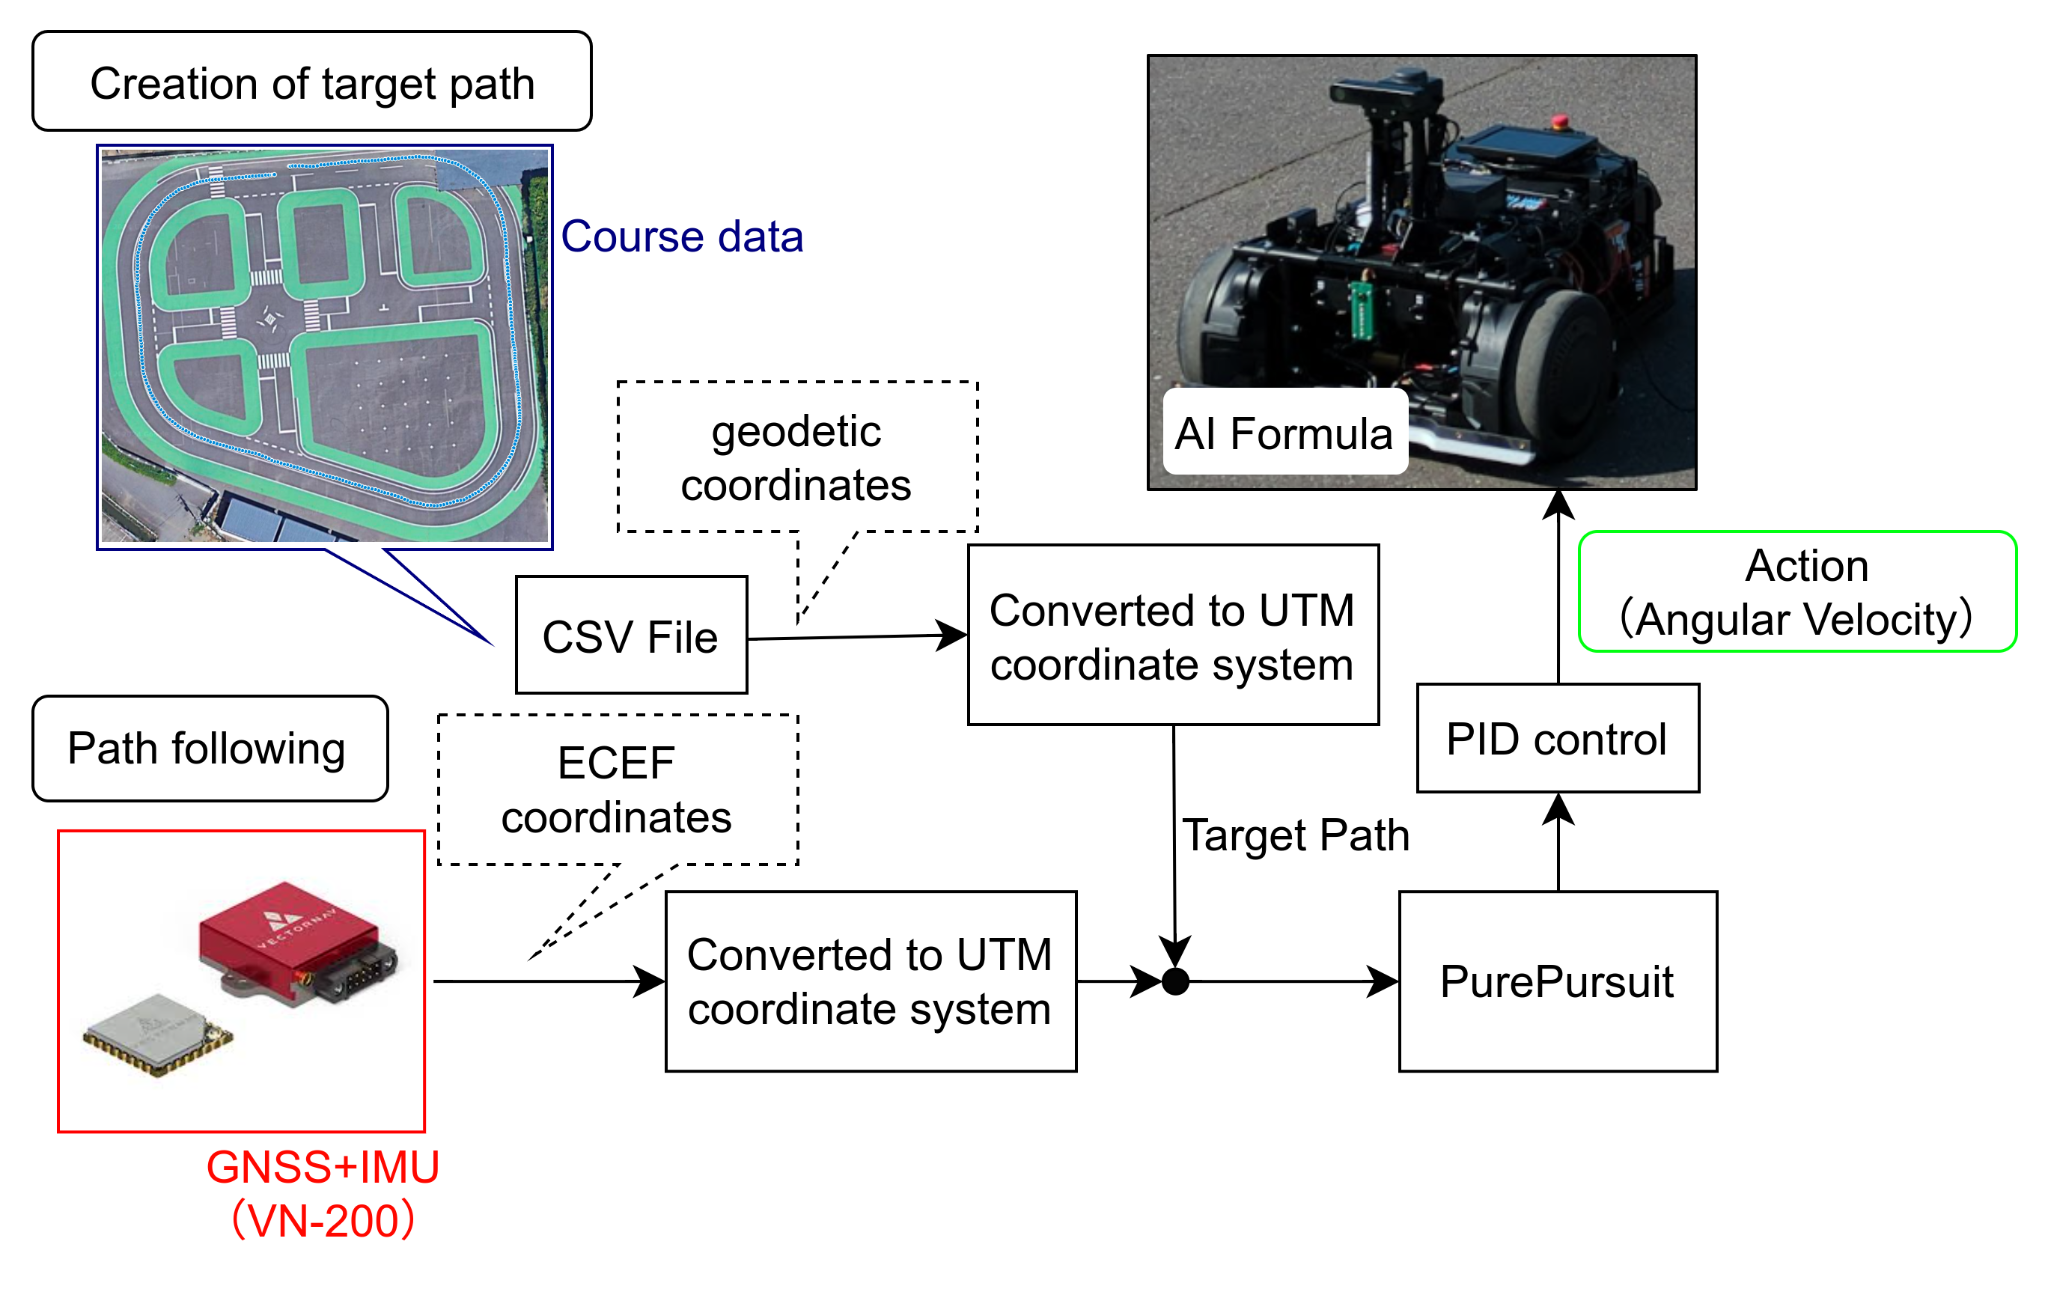
\includegraphics[keepaspectratio, scale=0.2]
      {images/system.png}
 \caption{Path-following system}
 \label{fig:Path-following system}
\end{figure}

\begin{table}[H]
     \centering
     \caption{Experimental device}
     \begin{tabular}{cclll}
     \cline{1-2}
     computer             & Jetson AGX Orin &  &  &  \\
     OS                   & Jetpack 5.1.2   &  &  &  \\
     ROS 2                & foxy            &  &  &  \\
                          &                 &  &  &  \\
                          &                 &  &  &  \\
                          &                 &  &  &  \\
     \multicolumn{1}{l}{} &                 &  &  &  \\
     \multicolumn{1}{l}{} &                 &  &  & 
     \end{tabular}
\end{table}

本研究で開発した経路追従ソフトウェアは事前に用意した目標経路に沿って追従する動作を行う.
本実験で使用する目標経路は実験当日にAIモビリティパーク紫峰で中央の白線に沿うように手動走行を行い, GNSSから得たデータを基に作成した.
Fig.6.3に作成した目標経路をGoogle Map上にプロットした図を示す.

\begin{figure}[H]
  \centering
 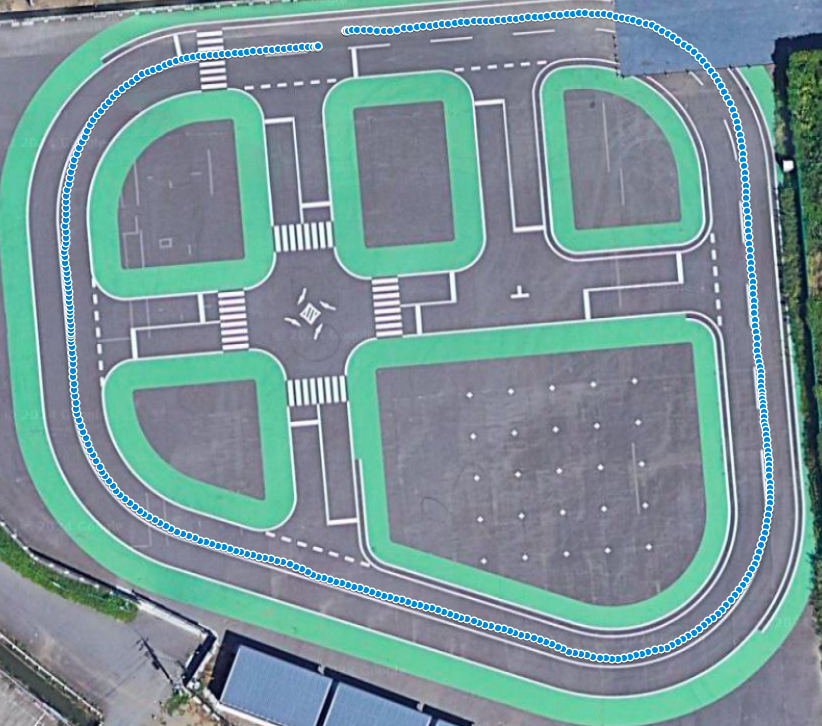
\includegraphics[keepaspectratio, scale=0.4]
      {images/targetpath.png}
 \caption{Aerial view and mobility perspective of the course}
 \label{fig:course}
\end{figure}

\section{実験内容}
本実験では, 開発した経路追従ソフトウェアの検証をするために, 以下の2つの実験を行う.
\begin{table}[H]
     \centering
     \begin{tabular}{lcl}
         $実験1$ &  & 低速域での経路追従ソフトウェアの初期検証 \\
         $実験2$ &  & 高速域での経路追従ソフトウェアの検証 \\
     \end{tabular}
\end{table}
% 実験1 低速域での経路追従ソフトウェアの初期検証
% 実験2 高速域での経路追従ソフトウェアの検証
実験1では, 低速域で走行させることにより開発した経路追従ソフトウェアの初期検証を行う.
実験2では, 高速域で走行させることにより低速域で走行した時との挙動の比較を行う.

Fig.6.4の丸で示された位置から矢印に沿うルートでAIモビリティパーク紫峰の外周を一周させる.
制御パラメータは以下とし, 目標速度は一定とする.

\begin{figure}[H]
  \centering
 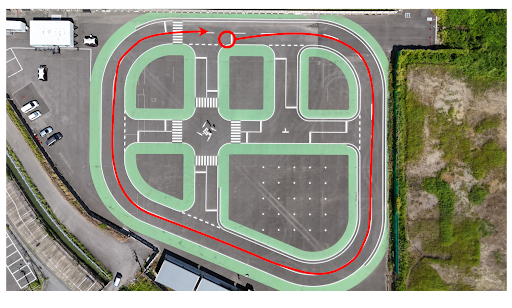
\includegraphics[keepaspectratio, scale=0.6]
      {images/AIFormulapath.png}
 \caption{Experiment path}
 \label{fig:path}
\end{figure}

\begin{table}[H]
     \centering
     \begin{tabular}{lcl}
         $linear\_vel$ & : & 目標速度 [m/s] \\
         $interval\_ms$ & : & 制御周期 [ms] \\
         $p\_gain$ & : & p制御のゲイン\\
         $i\_gain$ & : & i制御のゲイン\\
         $d\_gain$ & : & d制御のゲイン\\
     \end{tabular}
\end{table}

\subsection{実験1  低速域での経路追従ソフトウェアの初期検証}
開発した経路追従ソフトウェアの初期検証を行うために, 目標速度3.0[m/s]で実験を行う.
走行時のパラメータをTable.6.3に示す.
\begin{table}[H]
     \centering
     \caption{Experiment1 parameters}
     \begin{tabular}{cclll}
     \multicolumn{1}{c|}{linear\_vel}     & 3.0  &  &  &  \\
     \multicolumn{1}{c|}{interval\_ms}    & 50   &  &  &  \\
     \multicolumn{1}{c|}{p\_gain}          & 0.8  &  &  &  \\
     \multicolumn{1}{c|}{i\_gain}          & 0.0  &  &  &  \\
     \multicolumn{1}{c|}{d\_gain}          & 0.0 &  &  &  \\
     \multicolumn{1}{l}{}                 &      &  &  &  \\
     % \multicolumn{1}{l}{}                 &      &  &  & 
     \end{tabular}
\end{table}

\subsection{実験2  高速域での経路追従ソフトウェアの検証}
目標速度6.0[m/s]で実験を行う.
走行時のパラメータをTable.6.4に示す.

\begin{table}[H]
     \centering
     \caption{Experiment1 parameters}
     \begin{tabular}{cclll}
     \multicolumn{1}{c|}{linear\_vel}     & 6.0  &  &  &  \\
     \multicolumn{1}{c|}{interval\_ms}    & 50   &  &  &  \\
     \multicolumn{1}{c|}{p\_gain}          & 1.0  &  &  &  \\
     \multicolumn{1}{c|}{i\_gain}          & 0.0  &  &  &  \\
     \multicolumn{1}{c|}{d\_gain}          & 0.15 &  &  &  \\
     \multicolumn{1}{l}{}                 &      &  &  &  \\
     \multicolumn{1}{l}{}                 &      &  &  & 
     \end{tabular}
\end{table}

\newpage

\section{実験結果}

\subsection{実験1   低速域での経路追従ソフトウェアの初期検証}
実験の結果, 目標並進速度3[m/s]で経路から外れること無くコースを一周することができた.
実験時の走行経路と目標経路の軌跡をFig.6.5に示す.
走行経路は走行時のGNSSデータを基準に求めている.
また, 目標経路との誤差の遷移をFig.6.6に示す.
最後に評価項目の結果をTable.6.5に示す.

\begin{figure}[H]
     \centering
    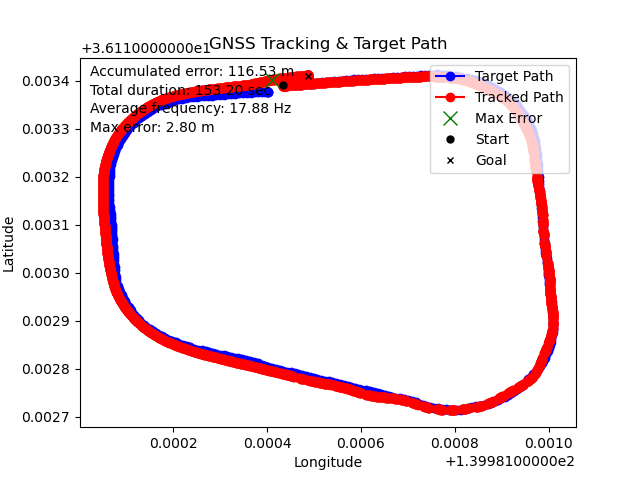
\includegraphics[keepaspectratio, scale=0.55]
         {images/3msIAE.png}
    \caption{Trajectory of travel route and target route}
    \label{fig:path}
\end{figure}

\begin{figure}[H]
     \centering
    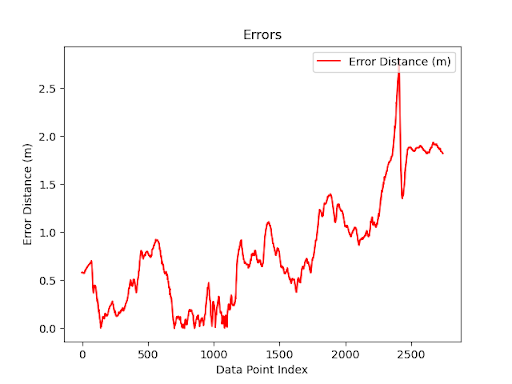
\includegraphics[keepaspectratio, scale=0.7]
         {images/3mserror.png}
    \caption{Transition of error from the target path}
    \label{fig:path}
\end{figure}

\begin{table}[H]
     \centering
     \caption{Evaluation item}
     \begin{tabular}{cclll}
     \multicolumn{1}{c|}{ゴールするまでの時間{[}s{]}}           & 153   &  &  &  \\
     \multicolumn{1}{c|}{積分絶対値誤差{[}m·s{]}} & 116.53 &  &  &  \\
     \multicolumn{1}{c|}{追従誤差の最大値{[}m{]}} & 2.8 &  &  &  \\
                                                &      &  &  &  \\
                                                &      &  &  &  \\
     \multicolumn{1}{l}{}                       &      &  &  &  \\
     \multicolumn{1}{l}{}                       &      &  &  & 
     \end{tabular}
\end{table}

\subsection{実験2   高速域での経路追従ソフトウェアの検証}
実験の結果, 目標並進速度6[m/s]で経路から外れること無くコースを一周することができた.
コースの初めのカーブ後の道で蛇行する動きを見せたものの, 経路から外れることなく周回することができた.
実験時の走行経路と目標経路の軌跡をFig.6.7に示す.
また, 目標経路との誤差の遷移をFig.6.8に示す.
最後に評価項目の結果をTable.6.6に示す.

\begin{figure}[H]
     \centering
    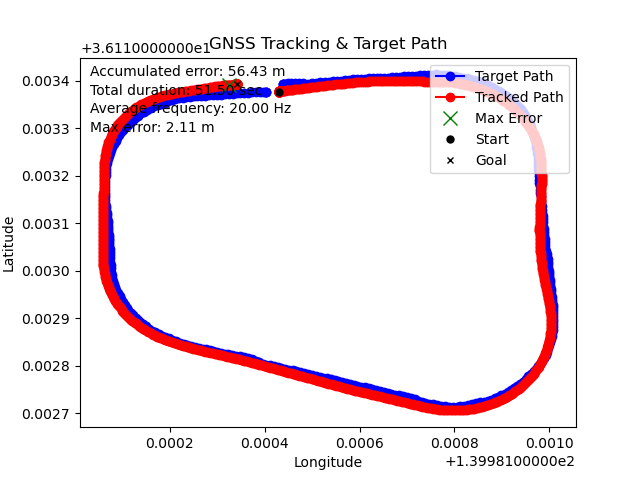
\includegraphics[keepaspectratio, scale=0.55]
         {images/6msIAE.png}
    \caption{Trajectory of travel route and target route}
    \label{fig:path}
\end{figure}

\begin{figure}[H]
     \centering
    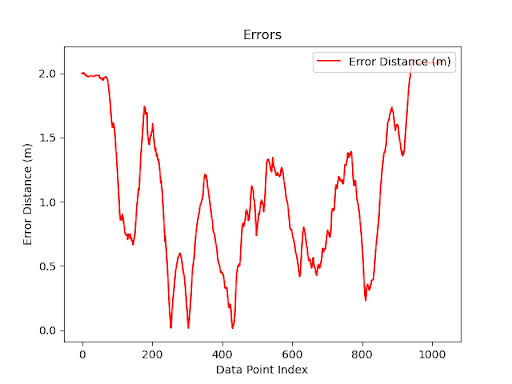
\includegraphics[keepaspectratio, scale=0.7]
         {images/6mserror.png}
    \caption{Transition of error from the target path}
    \label{fig:path}
\end{figure}

\begin{table}[H]
     \centering
     \caption{Evaluation item}
     \begin{tabular}{cclll}
     \multicolumn{1}{c|}{ゴールするまでの時間{[}s{]}}           & 51   &  &  &  \\
     \multicolumn{1}{c|}{積分絶対値誤差{[}m·s{]}} & 56.43 &  &  &  \\
     \multicolumn{1}{c|}{追従誤差の最大値{[}m{]}} & 2.11 &  &  &  \\
                                                &      &  &  &  \\
                                                &      &  &  &  \\
     \multicolumn{1}{l}{}                       &      &  &  &  \\
     \multicolumn{1}{l}{}                       &      &  &  & 
     \end{tabular}
\end{table}

開発した経路追従ソフトウェアを実環境で検証した.
検証の結果, 開発した経路追従ソフトウェアは目標経路を適切に追従し, 高速域においても経路から逸脱することなく走行可能であることが確認された.
低速域と高速域における追従誤差を比較すると, 高速域では一部蛇行挙動が見られたが, 大きな逸脱は発生しなかった.